% Construction : A = (0, 0), B = (4, 0), C = (0, 3), D = (3, 0), E = (0 ; 2,25).
% Une unité vaut 1,6 cm : AB = 6,4 ; AC = 4,8 ; AD = 4,8 ; AE = 3,6 ; BC = 8 ; DE = 6.
% Les points A, D, B sont alignés, ainsi que A, E, C ; (DE) et (BC) ont la même
% pente, \(-3/4\), et le rapport de Thalès vaut 0,75.
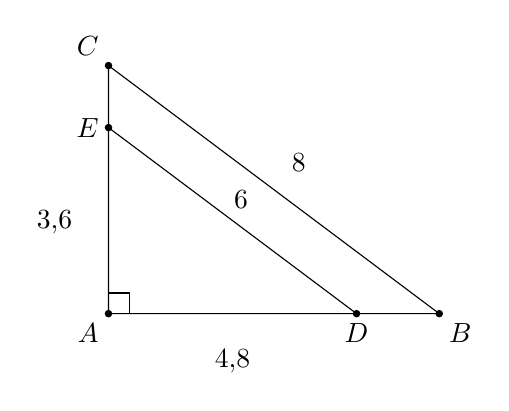
\begin{tikzpicture}[scale=1.05]
  \coordinate (A) at (0, 0);
  \coordinate (B) at (4, 0);
  \coordinate (C) at (0, 3);
  \coordinate (D) at (3, 0);
  \coordinate (E) at (0, 2.25);
  \draw (A) -- (B) -- (C) -- cycle;
  \draw (D) -- (E);
  \draw (0.25, 0) -- (0.25, 0.25) -- (0, 0.25);
  \foreach \p in {A, B, C, D, E} \fill (\p) circle (1.3pt);
  \node[below left]  at (A) {$A$};
  \node[below right] at (B) {$B$};
  \node[above left]  at (C) {$C$};
  \node[below] at (D) {$D$};
  \node[left]  at (E) {$E$};
  \node[below] at (1.5, -0.32) {$4{,}8$};
  \node[left]  at (-0.32, 1.1) {$3{,}6$};
  \node[above right] at (1.4, 1.15) {$6$};
  \node[above right] at (2.1, 1.6) {$8$};
\end{tikzpicture}
